%\begin{document}
\chapter{基于先验信息MMSE准则的线性Turbo均衡算法}
\thispagestyle{empty}
%=========================================================================
\section{MMSE均衡算法}
如图\ref{fig:3.1}为水声相干通信系统的传输模型,包括发射部分,传输部分以及接收部分。在接收部分中又包含了均衡器、译码器以及信道估计器。本章的重点在于均衡算法,因此主要关注SISO均衡器。

现在把图\ref{fig:2.4}中的接收部分单独拿出来,并采用基于先验信息MMSE准则的线性Turbo均衡器(MMSE-LE)代替图\ref{fig:2.4}中的SISO均衡器。如图\ref{fig:3.1}

\begin{figure}[htb]
  \begin{center}
    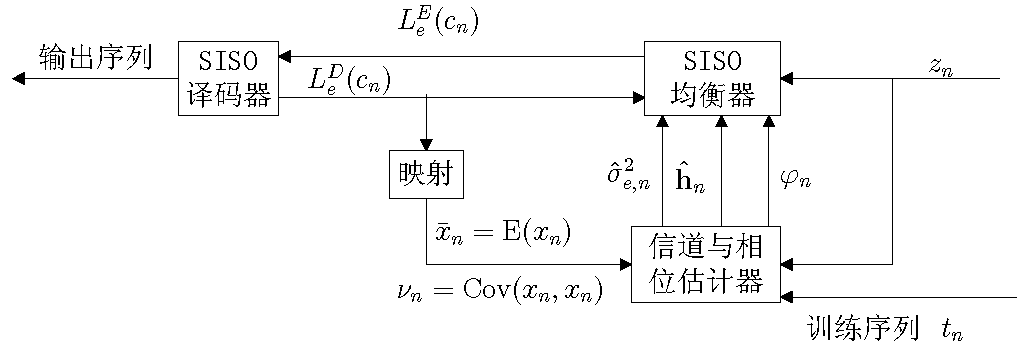
\includegraphics[width=0.8\textwidth]{images/mmse2.pdf}
  \end{center}
  \caption{基于MMSE-LE的接收端}
  \label{fig:3.1}
\end{figure}

从图\ref{fig:3.1}中可以看出,接收符号$z_n$以及SISO译码器的软输出作为MMSE-LE的输入,并给SISO译码器提供软信息,从而构成一个回路,通过不断的迭代来提高均衡和译码的性能。为了专注于均衡算法部分,将图\ref{fig:3.1}中与均衡无关的部分暂且去除,从而得到图\ref{fig:3.2}

\begin{figure}[htb]
  \begin{center}
    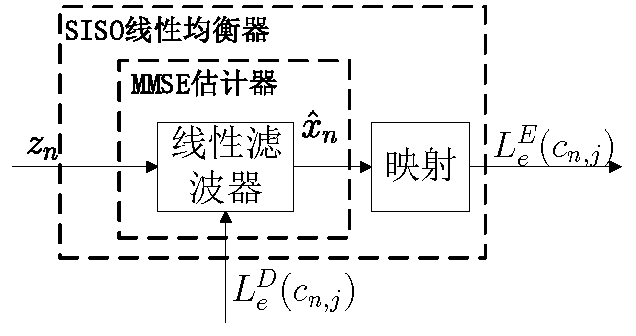
\includegraphics[width=0.8\textwidth]{images/mmse_LE.pdf}
  \end{center}
  \caption{MMSE-LE内部结构框图}
  \label{fig:3.2}
\end{figure}

从图\ref{fig:3.2}中可以看出,MMSE-LE包括两个部分,
\begin{enumerate}
    \item MMSE估计器
    \item 映射
\end{enumerate}
下面就从这两个方面对MMSE-LE算法进行详细介绍。
\subsection{MMSE估计器}
利用长度为$N=N_1+N_2+1$的接收符号序列$\mathbf{z}_n=[z_{n-N_2},z_{n-N_2+1},\cdots,z_{n+N_1}]$来计算发送符号$x_n$的线性估计值$\hat{x}_n$:
\begin{eqnarray}
    \hat{x}_n=\mathbf{a}_n^{\mathrm{H}}\mathbf{z}_n+b_n
    \label{equ:3.1}
\end{eqnarray}
其中$\mathbf{a}_n\overset{\Delta}{=}[a_{n,N_2}^*,a_{n,N_2-1}^*,\cdots,a_{n,-N_1}^*]^{\mathrm{T}},a_{n,k}\in
\mathbb{C}$为线性滤波器的系数,$b_n\in
\mathbb{C}$是在给定先验信息的情况下,随机变量$x_n$的非零均衡的时变偏移补偿。$N_1$和$N_2$为线性滤波器的非因果和因果长度。$N$为滤波器的总长度。

当允许$\mathbf{a}_n$和$b_n$都随$n$变化时,通过最小均方误差准则(MMSE),选择
\begin{eqnarray}
    \begin{array}{l@{\;=\;}l}
        \mathbf{a}_n&\mathrm{Cov}(\mathbf{z}_n,\mathbf{z}_n)^{-1}\mathrm{Cov}(\mathbf{z}_n,x_n)\\   
        b_n&\mathrm{E}(x_n)-\mathbf{a}_n^{\mathrm{H}}\mathrm{E}(\mathbf{z}_n)
    \end{array}
    \label{equ:3.2}
\end{eqnarray}
来最小化$\mathrm{E}(|x_n-\hat{x}_n|^2)$,从而得出:
\begin{eqnarray}
    \hat{x}_n=\mathrm{E}(x_n)+\mathrm{Cov}(x_n,\mathbf{z}_n)\mathrm{Cov}(\mathbf{z}_n,\mathbf{z}_n)^{-1}(\mathbf{z}_n-\mathrm{E}(\mathbf{z}_n))
    \label{equ:3.3}
\end{eqnarray}
这种算法称作为最小均方误差算法(MMSE)。

上式中,$\mathbf{z}_n$为接收符号序列:
\begin{eqnarray}
    \mathbf{z}_n=\mathbf{H}_n\mathbf{x}_n+\boldsymbol{\omega}_n
    \label{equ:3.4}
\end{eqnarray}
其中,$\mathbf{x}_n\overset{\Delta}{=}[x_{n-N_2-M+1},x_{n-N_2-M+2},\cdots,x_{n+N_1}]^{\mathrm{T}}$为发送符号序列,$H$为$N\times
(N+M-1)$的信道矩阵,$M$为信道冲激响应长度:
\begin{eqnarray}
\mathbf{H}_n\overset{\Delta}{=}\begin{bmatrix}
 h_{M-1}&h_{M-2}  &\cdots  & h_0 & 0 & \cdots &  &0 \\ 
 &h_{M-1}  & h_{M-2} & \cdots & h_0 & 0 & \cdots &0 \\ 
 &  &  &  \ddots&  &  &  & \\ 
 0&  & \cdots & 0 & h_{M-1} &h_{M-2}  &\cdots  & h_0
\end{bmatrix}    
    \label{equ:3.5}
\end{eqnarray}
$\omega_n$为均值为$0$,方差为$\sigma_{\omega,n}^2$的高斯白噪声。

假设噪声$\omega_n$是独立同分布的(i.i.d),可以得到:
\begin{eqnarray}
    \begin{array}{r@{\;=\;}l}
        \mathrm{E}(\mathbf{z}_n)&\mathbf{H}_n\mathrm{E}(\mathbf{x}_n)\\
        \mathrm{Cov}(x_n,\mathbf{z}_n)&\mathrm{Cov}(x_n,x_n)[\mathbf{0}_{1\times(N_2+M-1)}\;1\;\mathbf{0}_{1\times
        N_1}]\mathbf{H}_n^{\mathrm{H}}\\
        \mathrm{Cov}(\mathbf{z}_n,\mathbf{z}_n)&\sigma_{\omega,n}^2\mathbf{I}_N+\mathbf{H}_n\mathrm{Cov}(\mathbf{x}_n,\mathbf{x}_n)\mathbf{H}_n^{\mathrm{H}}\\
    \end{array}
    \label{equ:3.6}
\end{eqnarray}

由于比特$c_{n,j}$是独立同分布的,进而$x_n$也是独立的,从而可以得出,对于$n,m,n\neq
m$的情况下,$\mathrm{Cov}(x_n,x_m)=0$。所以协方差矩阵$\mathrm{Cov}(\mathbf{x}_n,\mathbf{x}_n)$只有在主对角线上式非零值。

如图\ref{fig:3.1},为了计算法$\mathbf{a}_n,b_n$,利用译码器反馈软信息$L_e^{\mathrm{D}}(c_{n,j})$可得随机变量$x_n$的先验信息和方差为:
\begin{eqnarray}
    \begin{array}{l@{\overset{\Delta}{=}}l}
        \bar{x}_n&\mathrm{E}(x_n)=\displaystyle\sum_{\alpha_i\in
        \mathcal{S}}\alpha_i\cdot P(x_n=\alpha_i)\\
        \upsilon_n&\mathrm{Cov}(x_n,x_n)=\left(\displaystyle\sum_{\alpha_i\in
        \mathcal{S}}|\alpha_i|^2\cdot P(x_n=\alpha_i)\right)-|\bar{x}_n|^2
    \end{array}
    \label{equ:3.7}
\end{eqnarray}
式\ref{equ:3.5}中概率$P(c_{n,j})$是对数似然比$L_e^{\mathrm{D}}(c_{n,j})$的函数,
\begin{eqnarray}
    \begin{array}{l@{\;=\;}l}
        \displaystyle
        P(x_n=\alpha_i)&\displaystyle\prod_{j=1}^{Q}P(c_{n,j}=s_{i,j})\\
        &\displaystyle\prod_{j=1}^Q1/2\cdot(1+\tilde{s}_{i,j}\cdot\tanh(L_e^{\mathrm{D}}(c_{n,j}/2)))
    \end{array}
    \label{equ:3.8}
\end{eqnarray}
其中
\begin{eqnarray}
    \tilde{s}_{i,j}\overset{\Delta}{=}
    \left\{
    \begin{matrix}
        +1&s_{i,j}=0\\
        -1&s_{i,j}=1
    \end{matrix}
    \right.
    \label{equ:3.9}
\end{eqnarray}

如果采用表\ref{tab:3.1}的映射方式,
\begin{table}[hbt]
  \centering
  \caption{QPSK映射方式}
  \label{tab:3.1}
  \begin{threeparttable}
  \begin{tabular}{ccccc}
    \hline
    $i$&$1$&$2$&$3$&$4$\\
    \hline
    $s_{i,1}\,s_{i,2}$&$00$&$10$&$01$&$11$\\
    $\alpha_i$&$(+1+\imath)/\sqrt{2}$&$(-1+\imath)/\sqrt{2}$&$(+1-\imath)/\sqrt{2}$&$(-1-\imath)/\sqrt{2}$\\
    \hline
  \end{tabular}
\end{threeparttable}
\end{table}
那么,$\bar{x}_n$和$\upsilon_n$的求解可以简化为表\ref{tab:3.2}
\begin{table}[hbt]
  \centering
  \caption{从$L_e^{\mathrm{D}}(c_{n,j})$求解$\bar{x}_n$和$\upsilon_n$}
  \label{tab:3.2}
  \begin{threeparttable}
  \begin{tabular}{c}
    \hline
    \heiti QPSK:\\
    \hline
    $\bar{x}_n=1/\sqrt{2}\cdot(\tanh(L_e^{\mathrm{D}}(c_{n,1})/2)+\tanh(L_e^{\mathrm{D}}(c_{n,2})/2)\imath)$\\
    $\upsilon_n=1-|\bar{x}_n|^2$\\
    \hline
  \end{tabular}
\end{threeparttable}
\end{table}

利用$\bar{x}_n$和$\upsilon_n$给出以下定义:
\begin{eqnarray}
    \begin{array}{l@{\overset{\Delta}{=}}l}
        \bar{z}_n&\mathrm{E}(z_n)=\displaystyle\sum_{k=0}^{M-1}h_k\bar{x}_{n-k}\\
        \bar{\mathbf{z}}_n&\mathrm{E}(\mathbf{z}_n)=[\bar{z}_{n-N_2},\bar{z}_{n-N_2+1},\cdots,\bar{z}_{n+N_1}]^{\mathrm{T}}\\
        \mathbf{V}_n&\mathrm{Cov}(x_n,x_n)=\mathrm{diag}(\upsilon_{n-M-N_2+1},\cdots,\upsilon_{n+N_1})\\
        \mathbf{s}_n&\mathbf{H}_n[\mathbf{0}_{1\times(N_2+M-1)}\;1\;\mathbf{0}_{1\times
        N_1}]^{\mathrm{T}}\\
        \boldsymbol{\Sigma}_n&\mathrm{Cov}(\mathbf{z}_n,\mathbf{z}_n)=(\sigma_{\omega,n}^2\mathbf{I}_N+\mathbf{H}_n\mathbf{V}_n\mathbf{H}_n^{\mathrm{H}})\\
    \end{array}
    \label{equ:3.10}
\end{eqnarray}

因此,估计值$\hat{x}_n$如下:
\begin{eqnarray}
    \hat{x}_n=\bar{x}_n+\mathbf{a}_n^{\mathrm{H}}(\mathbf{z}-\bar{\mathbf{z}}_n)=\bar{x}_n+\sum_{k=-N_1}^{N_2}a_{n,k}\cdot(z_{n-k}-\bar{z}_{n-k})
    \label{equ:3.11}
\end{eqnarray}
其中$\mathbf{a}_n=\upsilon_n\boldsymbol{\Sigma}^{-1}\mathbf{s}_n$,这个方程等价于$\mathbf{z}_n-\bar{\mathbf{z}}_n$经过一个线性滤波器,其滤波系数$f_{n,k},\,k=-N_1,1-N_1,\cdots,N_2$,具体如下:
\begin{eqnarray}
    \mathbf{f}_n=[f_{n,N_2}^*,f_{n,N_2-1}^*,\cdots,f_{n,-N_1}^*]^{\mathrm{T}}\overset{\Delta}{=}\boldsymbol{\Sigma}_n^{-1}\mathbf{s}_n
    \label{equ:3.12}
\end{eqnarray}
乘以$\upsilon_n$并加上$\bar{x}_n$可以得到估计符号如下:
\begin{eqnarray}
    \hat{x}_n=\bar{x}_n+\upsilon_n\cdot\mathbf{f}_n^{\mathrm{H}}(\mathbf{z}_n-\bar{\mathbf{z}}_n)
    \label{equ:3.13}
\end{eqnarray}
然而,$\hat{x}_n$通过$\bar{x}_n$和$\upsilon_n$依赖$L_e^{\mathrm{D}}(c_{n,j})$,这违背了求解外部信息时不能依赖先验信息的原则。为了使$\hat{x}_n$独立于$L_e^{\mathrm{D}}(c_{n,j})$,在计算$\hat{x}_n$的时候,将$L_e^{\mathrm{D}}(c_{n,j}),\,j=1,\cdots,Q$都设置为$0$,从而$\bar{x}_n=0$且$\upsilon_n=1$。式\ref{equ:3.13}可以改写如下:
\begin{eqnarray}
    \begin{array}{c}
    {\mathbf{f}}'_n\overset{\Delta}{=}\mathbf{f}_n|_{\upsilon_n=1}=(\boldsymbol{\Sigma}_n+(1-\upsilon_n)\mathbf{s}_n\mathbf{s}_n^{\mathrm{H}})^{-1}\mathbf{s}_n\\
    \hat{x}_n=0+1\cdot{{\mathbf{f}}'}_n^{\mathrm{H}}(\mathbf{z}_n-\bar{\mathbf{z}}_n+(\bar{x}_n-0)\mathbf{s}_n)
\end{array}
    \label{equ:3.14}
\end{eqnarray}
利用逆矩阵定理,可以得知${\mathbf{f}}'_n$是$\mathbf{f}_n$的伸展版,可以表示如下:
\begin{eqnarray}
    \begin{array}{l@{\;=\;}l}
        {\mathbf{f}}'_n&(\boldsymbol{\Sigma}_n^{-1}-\boldsymbol{\Sigma}_n^{-1}\mathbf{s}_n((1-\upsilon_n)^{-1}+\mathbf{s}_n\boldsymbol{\Sigma}_n^{-1}\mathbf{s}_n)^{-1}\mathbf{s}_n^{\mathrm{H}}\boldsymbol{\Sigma}_n^{-1})\mathbf{s}_n\\
        &\mathbf{f}_n-\mathbf{f}_n((1-\upsilon_n)^{-1}+\mathbf{f}_n^{\mathrm{H}}\mathbf{s}_n)^{-1}\mathbf{f}_n^{\mathrm{H}}\mathbf{s}_n\\
        &(1+(1-\upsilon_n)^{-1}+\mathbf{f}_n^{\mathrm{H}}\mathbf{s}_n)^{-1}\mathbf{f}_n
    \end{array}
    \label{equ:3.15}
\end{eqnarray}
因此,估计符号$\hat{x}_n$可以改写如下:
\begin{eqnarray}
    \hat{x}_n=K_n\cdot\mathbf{f}_n^{\mathrm{H}}(\mathbf{z}_n-\bar{\mathbf{z}}_n+\bar{x}_n\mathbf{s}_n)
    \label{equ:3.16}
\end{eqnarray}
其中,$K_n\overset{\Delta}{=}(1+(1-\upsilon_n)\mathbf{f}_n^{\mathrm{H}}\mathbf{s}_n)^{-1}$
\subsection{映射}
上一节已经得到了发送符号的估计值$\hat{x}_n$,对于传统线性均衡器来说,其结果可以直接给译码器,最后得到译码结果。但是,由于采用的是Turbo均衡算法,因此译码器采用软输入软输出算法,因此,需要关于发送符号的软信息。具体可以看图\ref{fig:3.2}。

基于MMSE准则的线性Turbo均衡器计算其后验对数似然比LLR值:
\begin{eqnarray}
    \begin{array}{l@{\;\overset{\Delta}{=}\;}l}
        L(c_{n,j}|\hat{x}_n)&\ln\frac{\displaystyle P(c_{n,j}=0|\hat{x}_n)}{\displaystyle P(c_{n,j}=1|\hat{x}_n)}\\
        &\ln\frac{\displaystyle\sum_{\forall\mathbf{c}_n:c_{n,j}=0}p(\hat{x}_n|\mathbf{c}_n)P(\mathbf{c}_n)}{\displaystyle\sum_{\forall\mathbf{c}_n:c_{n,j}=1}p(\hat{x}_n|\mathbf{c}_n)P(\mathbf{c}_n)}
    \end{array}
    \label{equ:3.17}
\end{eqnarray}
上式可以分解如下:
\begin{eqnarray}
      \underbrace{\ln\frac{\displaystyle\sum_{\forall\mathbf{c}_n:c_{n,j}=0}p(\hat{x}_n|\mathbf{c}_n)\prod_{\forall
    {j}'\neq
    j}P(c_n,{j}')}{\displaystyle\sum_{\forall\mathbf{c}_n:c_{n,j}=1}p(\hat{x}_n|\mathbf{c}_n)\prod_{\forall
    {j}'\neq j}P(c_n,{j}')}}_{L_e^{\mathrm{E}}(c_{n,j})}+L_a(c_{n,j})    
    \label{equ:3.18}
\end{eqnarray}
其中,$L_a(c_{n,j})$为上一次译码器反馈的外部信息$L_e^{\mathrm{D}}(c_{n,j})$,作为均衡器的先验信息。$L_e^{\mathrm{E}}(c_{n,j})$是均衡器输出的软信息,也是要通过$\hat{x}_n$映射得到的。

假设PDF
$p(\hat{x}_n|\mathbf{c}_n=\mathbf{s}_i)=p(\hat{x}_n|x_n=\alpha_i),\,i=1,2,\cdots,2^Q$是均值为$\mu_{n,i}\overset{\Delta}{=}\mathrm{E}(\hat{x}_n|x_n=\alpha_i)$,方差为$\sigma_{n,i}^2=\mathrm{Cov}(\hat{x}_n,\mathrm{x}_n|x_n=\alpha_i)$的高斯分布:
\begin{eqnarray}
    p(\hat{x}_n|\mathbf{c}_n=\mathbf{s}_i)\approx\phi_{\mu_{n,i},\sigma_{n,j}^2}(\hat{x}_n)
    \label{equ:3.19}
\end{eqnarray}
这个假设可以简化$L_e^{\mathrm{E}}(c_{n,j})$的计算,而且只应用于$\hat{x}_n$到$L_e^{\mathrm{E}}(c_{n,j})$的映射,因此性能损失是可以忽略不计的。而且发现$L_e^{\mathrm{E}}(c_{n,j})$或$L(c_{n,j}|\hat{x}_n)$对于小范围的性能损失的鲁棒性非常好。

$\hat{x}_n$的统计量$\mu_{n,i}$和$\sigma_{n,i}^2$如下:
\begin{eqnarray}
     \begin{array}{l@{\;=\;}l}
           \mu_{n,j}&\mathbf{f}_n^{\mathrm{H}}(\mathrm{E}(\mathbf{z}_n|x_n=\alpha_i)-\bar{\mathbf{z}}_n+\bar{x}_n\mathbf{s}_n)\\
           &\mathbf{f}_n^{\mathrm{H}}(\mathbf{H}_n\mathrm{E}(\mathbf{x}_n|x_n=\alpha_i)-\bar{\mathbf{z}}_n+\bar{x}_n\mathbf{s}_n)\\
           &\alpha_i\cdot\mathbf{f}^{\mathrm{H}}_n\mathbf{s}_n\\
           \sigma^2_{n,i}&\mathbf{f}^{\mathrm{H}}_n\mathrm{Cov}(\mathbf{z}_n,\mathbf{z}_n|x_n=\alpha_i)\mathbf{f}_n\\
           &\mathbf{f}_n^{\mathrm{H}}(\Sigma_n-\upsilon_n\mathbf{s}_n\mathbf{s}_n^{\mathrm{H}})\mathbf{f}_n\\
           &\mathbf{f}_n^{\mathrm{H}}\mathbf{s}_n-\upsilon_n\mathbf{f}_n^{\mathrm{H}}\mathbf{s}_n\mathbf{s}_n^{\mathrm{H}}\mathbf{f}_n
       \end{array}
           \label{equ:3.20}
\end{eqnarray}
从而得到:
\begin{eqnarray}
      \begin{array}{l@{\;=\;}l}
          L_e^{\mathrm{E}}(c_{n,j})& \ln\frac{\displaystyle\sum_{\forall \mathbf{s}_i:s_{i,j}=0}p(\hat{x}_n|\mathbf{c}_n=\mathbf{s}_i)\prod_{\forall {j}':{j}'\neq j}P(c_{n,{j}'}=s_{i,{j}'})}{\displaystyle\sum_{\forall \mathbf{s}_i:s_{i,j}=1}p(\hat{x}_n|\mathbf{c}_n=\mathbf{s}_i)\prod_{\forall {j}':{j}'\neq j}P(c_{n,{j}'}=s_{i,{j}'})}\\
        & \ln\frac{\displaystyle\sum_{\forall
         \mathbf{s}_i:s_{i,j}=0}\exp\left(-\rho_{n,j}+\sum_{\forall
         {j}':{j}'\neq j}\tilde{s}_{i,{j}'}L(c_{n,{j}'})/2\right
         )}{\displaystyle\sum_{\forall \mathbf{s}_i:s_{i,j}=1}\exp\left(-\rho_{n,j}+\sum_{\forall {j}':{j}'\neq j}\tilde{s}_{i,{j}'}L(c_{n,{j}'})/2\right)}\\
    \end{array}
    \label{equ:3.21}
\end{eqnarray}
其中,
\begin{eqnarray}
    \begin{array}{l@{\;=\;}l}
     \rho_{n,j}&\frac{\displaystyle|\bar{x}_n-\mu_{n,i}|^2}{\displaystyle\sigma^2_{n,i}}\\
     &\frac{\displaystyle|\mathbf{f}^{\mathrm{H}}_n(\mathbf{z}_n-\bar{\mathbf{z}}_n+\bar{x}_n\mathbf{s}_n)-\alpha_i\mathbf{f}^{\mathrm{H}}_n\mathbf{s}_n|^2}{\displaystyle\mathbf{f}^{\mathrm{H}}_n\mathbf{s}_n-\upsilon_n\mathbf{f}^{\mathrm{H}}_n\mathbf{s}_n\mathbf{s}_n^{\mathrm{H}}\mathbf{f}_n}
 \end{array} 
    \label{equ:3.22}
\end{eqnarray}

对于\ref{tab:3.1}的映射方式,则外部信息$L_e^{\mathrm{E}}(c_{n,j})$可以简化为:
\begin{table}[hbt]
  \centering
  \caption{$L_e^{\mathrm{E}}(c_{n,j})$的计算公式}
  \label{tab:3.3}
  \begin{threeparttable}
  \begin{tabular}{c}
    \hline
    \heiti QPSK\\
    \hline
    $L_e^{\mathrm{E}}(c_{n,1})=\sqrt{8}/(1-\upsilon_n\mathbf{s}_n^{\mathrm{H}}\mathbf{f}_n)\cdot\mathrm{Re}(\mathbf{f}_n^{\mathrm{H}}(\mathbf{z}_n-\bar{\mathbf{z}}_n+\bar{x}_n\mathbf{s}_n))$\\
    $L_e^{\mathrm{E}}(c_{n,2})=\sqrt{8}/(1-\upsilon_n\mathbf{s}_n^{\mathrm{H}}\mathbf{f}_n)\cdot\mathrm{Im}(\mathbf{f}_n^{\mathrm{H}}(\mathbf{z}_n-\bar{\mathbf{z}}_n+\bar{x}_n\mathbf{s}_n))$\\
    \hline
  \end{tabular}
\end{threeparttable}
\end{table}

如果先验信息不存在,也即是$L_e^{\mathrm{D}}(c_{n,j})=0$对所有的$n,j$,那么$\mathbf{f}_n$是固定的,不随时间而改变。在此条件下,$\bar{x}_n=0,\upsilon_n=1$,那么$\mathbf{f}_n$可以改写如下:
\begin{eqnarray}
    \mathbf{f}_{NA}\overset{\Delta}{=}\boldsymbol{\Sigma}_n^{-1}|_{\upsilon_n=1,\forall
    \,n}=(\sigma_{\omega}^2\mathbf{I}_N+\mathbf{H}_n\mathbf{H}_n^{\mathrm{H}})^{-1}\mathbf{s}_n
    \label{equ:3.23}
\end{eqnarray}
此式与传统的MMSE均衡器一样,NA代表的是“没有先验信息”。对于传统线性均衡器,可以采用最陡下降法来降低运算复杂度,然而本文采用的基于先验信息MMSE准则的线性Turbo均衡算法中,$\mathbf{f}_n$依赖于$\mathbf{H}_n$和$\mathbf{V}_n$,最陡下降法不能适用,因此必须计算矩阵的逆,直接实现此操作需要$N^3$的计算量。
\subsection{算法优化与总结}
分析$\boldsymbol{\Sigma}_n$的结构从而发展出一个快速递归求解$\mathbf{f}_n$的算法,此算法只需要$N^2$的计算量。很多关于自适应滤波器的文献\cite{Simon2001,strobach1986}都有相关的快速算法。本文主要参考文献\ncite{Tuchler2002a}中的快速算法。时间递归更新算法如下:
\begin{eqnarray}
    \boldsymbol{\Sigma}_n\overset{\Delta}{=}
    \begin{bmatrix}
        \sigma_{\mathrm{P}}&\boldsymbol{\sigma}_{\mathrm{P}}^{\mathrm{H}}\\
        \boldsymbol{\sigma}_{\mathrm{P}}&\boldsymbol{\Sigma}_{\mathrm{P}}
    \end{bmatrix}
    ,\qquad
    \boldsymbol{\Sigma}_{n+1}\overset{\Delta}{=}
    \begin{bmatrix}
        \boldsymbol{\Sigma}_{\mathrm{N}}&\boldsymbol{\sigma}_{\mathrm{N}}\\
        \boldsymbol{\sigma}_{\mathrm{N}}^{\mathrm{H}}&\sigma_{\mathrm{N}}
    \end{bmatrix}
    \label{equ:3.24}
\end{eqnarray}
其中,$\boldsymbol{\Sigma}_i,\,i\in\{P.N\}$是$(N-1)\times(N-1)$的矩阵,$\boldsymbol{\sigma}_i$是长度为$N-1$的列向量,$\sigma_i$则是标量。下标$P$代表当前“Present”时间$n$。而$N$代表下一“next”时间$n+1$。相似的,对于$\boldsymbol{\Sigma}_n,\boldsymbol{\Sigma}_{n+1}$的逆的划分如下:
\begin{eqnarray}
    \begin{array}{l@{\;\overset{\Delta}{=}\;}l@{\;\overset{\Delta}{=}\;}l}
        \boldsymbol{\Sigma}_n^{-1}&\mathbf{U}_n&
        \begin{bmatrix}
            u_{\mathrm{P}}&\mathbf{u}_{\mathrm{P}}^{\mathrm{H}}\\
            \mathbf{u}_{\mathrm{P}}&\mathbf{U}_{\mathrm{P}}\\
        \end{bmatrix}\\
        \boldsymbol{\Sigma}_{n+1}^{-1}&\mathbf{U}_{n+1}&
        \begin{bmatrix}
            \mathbf{U}_{\mathrm{N}}&\mathbf{u}_{\mathrm{N}}\\
            \mathbf{u}_{\mathrm{N}}^{\mathrm{H}}&u_{\mathrm{N}}
        \end{bmatrix}
    \end{array}
    \label{equ:3.25}
\end{eqnarray}
其中,用到了Hermitian矩阵的逆依然是Hermitian矩阵这一性质。从上式可以发现,$\boldsymbol{\Sigma}_{\mathrm{P}}$和$\boldsymbol{\Sigma}_{\mathrm{N}}$是一致的:
\begin{eqnarray}
    \boldsymbol{\Sigma}_{\mathrm{P}}=\boldsymbol{\Sigma}_{\mathrm{N}}=\sigma_{\omega,n}^2\mathbf{I}_{\mathrm{N}}+{\mathbf{H}}'_n\mathrm{diag}[\upsilon_{n-M+N_2+2},\cdots,\upsilon_{n+N_1}]{{\mathbf{H}}'}_n^{\mathrm{H}}
    \label{equ:3.26}
\end{eqnarray}
其中,${\mathbf{H}}'$是$(N-1)\times(N+M-2)$的信道卷积矩阵。基于这个事实,递归算法从$\mathbf{U}_n$计算$\boldsymbol{\Sigma}_n^{-1}$,并令$\boldsymbol{\Sigma}_{\mathrm{P}}^{-1}=\boldsymbol{\Sigma}_{\mathrm{N}}^{-1}$,进而从$\boldsymbol{\Sigma}_{\mathrm{N}}^{-1}$计算得到$\mathbf{U}_{n+1}$。

$\boldsymbol{\Sigma}_{n}$的子矩阵$\boldsymbol{\Sigma}_{\mathrm{P}}$的逆$\boldsymbol{\Sigma}_{\mathrm{P}}^{-1}$可以通过解$\boldsymbol{\Sigma}_{n}\mathbf{U}_n=\mathbf{I}_{\mathrm{N}}$方程得到:
\begin{eqnarray}
    \begin{array}{c}
        \boldsymbol{\Sigma}_{\mathrm{P}}\mathbf{U}_{\mathrm{P}}+\boldsymbol{\sigma}_{\mathrm{P}}\mathbf{u}_{\mathrm{P}}^{\mathrm{H}}=\mathbf{I}_{\mathrm{N}-1}\\
     \boldsymbol{\Sigma}_{\mathrm{P}}\mathbf{u}_{\mathrm{P}}+\boldsymbol{\sigma}_{\mathrm{P}}u_{\mathrm{P}}^{\mathrm{H}}=\mathbf{0}_{\mathrm{N}-1}\\
     \qquad\rightarrow\;\boldsymbol{\Sigma}_{\mathrm{P}}^{-1}=\mathbf{U}_{\mathrm{P}}-\mathbf{u}_{\mathrm{P}}\mathbf{u}_{\mathrm{P}}^{\mathrm{N}}/u_{\mathrm{P}}
    \end{array}
    \label{equ:3.27}
\end{eqnarray}

通过求解方程$\boldsymbol{\Sigma}_{n+1}\mathbf{U}_{n+1}=\mathbf{I}_{\mathrm{N}}$,可以用$\boldsymbol{\Sigma}_{\mathrm{N}}$,$\boldsymbol{\sigma}_{\mathrm{N}}$以及$\sigma_{\mathrm{N}}$来表示$\mathbf{U}_{\mathrm{N}}$和$\mathbf{u}_{\mathrm{N}}$:
\begin{eqnarray}
    \begin{array}{l@{\,}l}
        {{\boldsymbol{\sigma}}'}_{\mathrm{N}}^{-1}&\overset{\Delta}{=}\boldsymbol{\Sigma}_{\mathrm{N}}^{-1}\boldsymbol{\sigma}_{\mathrm{N}}\\
        u_{\mathrm{N}}&=1/(\sigma_{\mathrm{N}}-\boldsymbol{\sigma}_{\mathrm{N}}^{\mathrm{H}}{\boldsymbol{\sigma}}'_{\mathrm{N}})\\
        \mathbf{u}_{\mathrm{N}}&=-u_{\mathrm{N}}{\boldsymbol{\sigma}}'_{\mathrm{N}}\\
        \mathbf{U}_{\mathrm{N}}&=\boldsymbol{\Sigma}_{\mathrm{N}}^{-1}+u_{\mathrm{N}}{\boldsymbol{\sigma}}'_{\mathrm{N}}{{\boldsymbol{\sigma}}'}_{\mathrm{N}}^{\mathrm{H}}
    \end{array}
    \label{equ:3.28}
\end{eqnarray}
其中,利用中间向量${\boldsymbol{\sigma}}'_{\mathrm{N}}$来简化算法。矩阵$\boldsymbol{\Sigma}_{\mathrm{N}}^{-1}$和矩阵$\boldsymbol{\Sigma}_{\mathrm{P}}^{-1}$是相等的,而且$\boldsymbol{\sigma}_{\mathrm{N}}$和$\sigma_{\mathrm{N}}$可以利用式\ref{equ:3.12}和\ref{equ:3.27}得到:
\begin{eqnarray}
    \begin{bmatrix}
        \boldsymbol{\sigma}_{\mathrm{N}}\\
        \sigma_{\mathrm{N}}
    \end{bmatrix}
    =
    \begin{bmatrix}
        \mathbf{0}_{\mathrm{N}-1}\\
        \sigma_{\omega}^2
    \end{bmatrix}
    +\mathbf{H}_n\mathbf{V}_{n-1}\mathbf{H}_n^{\mathrm{H}}
    \begin{bmatrix}
        \mathbf{0}_{\mathrm{N}-1}\\
        1
    \end{bmatrix}
    \label{equ:3.29}
\end{eqnarray}

此时,可以利用$\mathbf{U}_{\mathrm{N}}$,$\mathbf{u}_{\mathrm{N}}$和$u_{\mathrm{N}}$计算出$\mathbf{U}_n$,从而形成完整的递归算法。当$\mathbf{f}_{n+1}=\boldsymbol{\Sigma}_{n+1}^{-1}\mathbf{s}_{n+1}$得到之后,就可以利用式\ref{equ:3.21}求解出外部信息$L_e^E(c_{n+1,j})$。

为了利用这种时间递归算法,$\mathbf{U}_n$在$n=1$的初始化值$\mathbf{U}_1=(\sigma_{\omega}\mathbf{I}_{\mathrm{N}}+\mathbf{H}_1\mathbf{V}_1\mathbf{H}_1^{\mathrm{H}})^{-1}$需要给出。由于算法在训练序列的时候就开始递归计算,因此$\mathbf{V}_1=0$,从而得到$\mathbf{U}_1=\sigma_{\omega}^{-2}\mathbf{I}_{\mathrm{N}}$。算法步骤总结如表\ref{tab:3.4}
\begin{longtable}{l}
  \caption{MMSE-LE递归算法总结}
  \label{tab:3.4}\\

  \endfirsthead

  \multicolumn{1}{c}{续表~\thetable\hskip1em MMSE-LE递归算法总结}

  \endhead
  
  \hline
  \multicolumn{1}{r}{续下页}
  \endfoot
  \endlastfoot
    \hline
    \begin{minipage}[tb]{15cm}
        \textbf{\xiaosan 输入:}
    \begin{itemize}
        \item[-]  星座图映射$\mathcal{S}={\alpha_1,\cdots,\alpha_{2^Q}}$,
        \item[-]  滤波器长度$N_1$和$N_2$,
        \item[-]  信道特征$h_k,k=0,\cdots,M-1$和$\sigma_{\omega,n}^2$,
        \item[-]  接收符号$z_n,n=1-N_2,\cdots,L+N_1$,
        \item[-]
            先验信息$L_e^{\mathrm{D}}(c_{n,j}),n=1-N_2+M+1,\cdots,L+N_1,j=1,\cdots,Q$,
    \end{itemize}
    \vspace{5mm}
\end{minipage}\\
    \hline
    \begin{minipage}[tb]{15cm}
        \textbf{\xiaosan 初始化:}
    \begin{itemize}
        \item[-]
            定义变量$\mathbf{f}=\mathbf{0}_{\mathrm{N}},\tilde{\mathbf{U}}=\mathbf{0}_{N\times(N-1)},$
            
            $\mathbf{u}={\mathbf{u}}'=\mathbf{0}_{\mathrm{N}-1},x=u=\mu=\rho_i=0,i=1,\cdots,2^Q$,
        \item[-]   计算$\bar{x}_n$和$\upsilon_n,n=1-N_2-M+1,\cdots,L+N_1$,
        \item[-]   计算$\bar{z}_n,n=1-N_2,\cdots,L+N_1$,
        \item[-]
            计算$\tilde{\mathbf{U}}=(\sigma_{\omega,n}^2\mathbf{I}_{\mathrm{N}}+\mathbf{H}_1\mathbf{V}_1\mathbf{H}_1^{\mathrm{H}})^{-1}$,
    \end{itemize}
    \vspace{5mm}
\end{minipage}\\
    \hline
    \begin{minipage}[tb]{15cm}
        \textbf{\xiaosan 均衡算法:}

     \quad FOR $n=1$ TO $L$ DO

     \qquad $\mathbf{f}=\tilde{\mathbf{U}}\mathbf{s}$,
     
     \qquad $\mu=\mathbf{f}^{\mathrm{H}}\mathbf{s}$,

     \qquad  $x=\mathbf{f}^{\mathrm{H}}(\mathbf{z}_n-\bar{\mathbf{z}}_n)+\bar{x}_n\mu$,

     \quad FOR $i=1$ TO $2^Q$ DO

     \qquad $\rho_i=|x-\alpha_i\mu|^2/(\mu-\mu^2)$,

     \quad END

     \quad FOR $j=1$ TO $Q$ DO

     \qquad $ L_e^{\mathrm{E}}(c_{n,j})=\ln\frac{\displaystyle\sum_{\forall
         \mathbf{s}_i:s_{i,j}=0}\exp\left(-\rho_{n,j}+\sum_{\forall
         {j}':{j}'\neq j}\tilde{s}_{i,{j}'}L(c_{n,{j}'})/2\right
         )}{\displaystyle\sum_{\forall
         \mathbf{s}_i:s_{i,j}=1}\exp\left(-\rho_{n,j}+\sum_{\forall
         {j}':{j}'\neq j}\tilde{s}_{i,{j}'}L(c_{n,{j}'})/2\right)}$
         
         \quad END

     \quad IF $n<L$ THEN

     \qquad
     $\begin{bmatrix}\mathbf{U}&\mathbf{u}\\\mathbf{u}^{\mathrm{N}}&u\end{bmatrix}=\tilde{\mathbf{U}}$,

     \qquad    $\mathbf{U}=\mathbf{U}-\mathbf{u}\mathbf{u}^{\mathrm{H}}/u$,

     \qquad
     $\begin{bmatrix}\mathbf{u}&u\end{bmatrix}=\begin{bmatrix}\mathbf{0}_{\mathrm{N}-1}\\\sigma_{\omega,n}^2\end{bmatrix}=\mathbf{H}_{n+1}\mathbf{V}_{n+1}\mathbf{H}_{n+1}^{\mathrm{H}}$,

        \qquad ${\mathbf{u}}'=\mathbf{U}\mathbf{u}$,

       \qquad  $u=1/(u-\mathbf{u}^{\mathrm{H}}{\mathbf{u}}')$,

       \qquad  $\mathbf{u}=-u{\mathbf{u}}'$,

       \qquad  $\mathbf{U}=\mathbf{U}+u{\mathbf{u}}'{\mathbf{u}}^{'H}$,

       \qquad  $\tilde{\mathbf{U}}=\begin{bmatrix}u &
             \mathbf{u}^{\mathrm{H}}\\\mathbf{u}& \mathbf{U}\end{bmatrix}$,

        \quad     END

         \quad    END
     \vspace{5mm}
 \end{minipage}\\
    \hline
\end{longtable}
\section{低复杂度近似算法}
为了进一步减少计算量,寻找不随$n$变化的滤波器系数$\mathbf{f}\overset{\Delta}{=}[f_{N_2}^*,f_{N_2-1}^*,\cdots,f_{-N_1}^*]$,提出MMSE均衡算法的低复杂度近似解决方案来代替式\ref{equ:3.13}获取$\hat{x}_n$。其中,利用$\boldsymbol{\Sigma}_n+(1-\upsilon_n)\mathbf{s}\mathbf{s}^{\mathrm{H}}$的时间平均值来代替变化值:
\begin{eqnarray}
    \begin{array}{l@{\,}l}
        {\mathbf{f}}'&\overset{\Delta}{=}\left(\frac{1}{L}\sum\limits_{n=1}^{L}\boldsymbol{\Sigma}_n+(1-\upsilon_n)\mathbf{s}\mathbf{s}^{\mathrm{H}}\gamma\right)\\
        &=(\sigma_{\omega,n}^2\mathbf{I}_{\mathrm{N}}+\mathbf{H}\bar{\mathbf{V}}\mathbf{H}^{\mathrm{H}}\gamma\gamma+(1-\bar{\upsilon})\mathbf{s}\mathbf{s}^{\mathrm{H}})^{-1}\mathbf{s}
    \end{array}
    \label{equ:3.30}
\end{eqnarray}
其中$\bar{\mathbf{V}}\overset{\Delta}{=}\frac{1}{L}\sum_{n=1}^L\mathbf{V}_n$和$\bar{\upsilon}=\frac{1}{L}=\sum_{n=1}^L\upsilon_n$。发送符号估计值$\hat{x}_n$可以改写成:
\begin{eqnarray}
    \hat{x}_n=\mathbf{f}^{'\mathbf{H}}(\mathbf{z}_n-\bar{\mathbf{z}}_n+\bar{x}_n\mathbf{s})
    \label{equ:3.31}
\end{eqnarray}
定义向量:
\begin{eqnarray}
    \mathbf{f}\overset{\Delta}{=}(\sigma_{\omega,n}^2\mathbf{I}_{\mathrm{N}}+\mathbf{H}\bar{\mathbf{V}}\mathbf{H}^{\mathrm{H}})^{-1}\mathbf{s}
    \label{equ:3.32}
\end{eqnarray}
与上面算法相类似,${\mathbf{f}}'$也是$\mathbf{f}$的伸展:
\begin{eqnarray}
    {\mathbf{f}}'=(1+(1-\bar{\upsilon})\mathbf{f}^{\mathrm{H}})^{-1}\mathbf{f}
    \label{equ:3.33}
\end{eqnarray}
$\hat{x}_n$的均值和方差可以计算如下:
\begin{eqnarray}
    \begin{array}{l@{\;=\;}l}
        \mu_{n,i}&K\cdot\mathbf{f}^{\mathrm{H}}(\mathrm{E}(\mathbf{z}_n|x_n=\alpha_i)-\bar{\mathbf{z}}_n+\bar{x}_n\mathbf{s})\\
        &K\cdot\alpha_i\cdot\mathbf{f}^{\mathrm{H}}\mathbf{s}\\
        \sigma_{n,i}^2&K^2\cdot\mathbf{f}^{\mathrm{H}}\mathrm{Cov}(\mathbf{z}_n,\mathbf{z}_n|x_n=\alpha_i)\mathbf{f}\\
        &K^2\cdot\mathbf{f}^{\mathrm{H}}(\boldsymbol{\Sigma}_n-\upsilon_n\mathbf{s}\mathbf{s}^{\mathrm{H}})\mathbf{f}
    \end{array}
    \label{equ:3.34}
\end{eqnarray}
其中$K\overset{\Delta}{=}(1+(1-\bar{\upsilon})\mathbf{s}^{\mathrm{H}}\mathbf{f})^{-1}$,从而得到:
\begin{eqnarray}
    \rho_{n,i}=\frac{|\mathbf{f}^{\mathrm{H}}(\mathbf{z}_n-\bar{\mathbf{z}}_n+\bar{x}_n\mathbf{s})-\alpha_i\mathbf{f}^{\mathrm{H}}\mathbf{s}|^2}{\mathbf{f}^{\mathrm{H}}(\sigma_{\omega,n}^2\mathbf{I}_{\mathrm{H}}+\mathbf{H}\mathbf{V}_n\mathbf{H}^{\mathrm{H}}-\upsilon_n\mathbf{s}\mathbf{s}^{\mathrm{H}})\mathbf{f}}
    \label{equ:3.35}
\end{eqnarray}
利用式\ref{equ:3.17}可以求出均衡器输出的外部软信息$L_e^E(c_{n,j})$。

对于$L$很长的情况下,$\bar{\mathbf{V}}$可以用$\bar{\upsilon}\mathbf{I}_{\mathrm{N+M}-1}$代替,而此中替换对于SISO均衡器的性能影响很小,因此可以简化$\mathbf{f}$为:
\begin{eqnarray}
    \hat{\mathbf{f}}\overset{\Delta}{=}(\sigma_{\omega,n}^2\mathbf{I}_{\mathrm{N}}+\bar{\upsilon}\mathbf{H}\mathbf{H}^{\mathrm{H}})^{-1}\mathbf{s}
    \label{equ:3.36}
\end{eqnarray}
$\rho_{n,i}$可以简化如下:
\begin{eqnarray}
    \begin{array}{c}
        \frac{\displaystyle
        |\mathbf{f}^{\mathrm{H}}(\mathbf{z}_n-\bar{\mathbf{z}}_n+\bar{x}_n\mathbf{s})-\alpha_i\mathbf{f}^{\mathrm{H}}\mathbf{s}|^2}{\displaystyle
        \mathbf{f}^{\mathrm{H}}(\sigma_{\omega,n}^2\mathbf{I}_{\mathrm{N}}+\mathbf{H}\mathbf{V}_n\mathbf{H}^{\mathbf{H}}-\upsilon_n\mathbf{s}\mathbf{s}^{\mathrm{H}})\mathbf{f}}\\
        \approx
        \frac{\displaystyle
        |\hat{\mathbf{f}}^{\mathrm{H}}(\mathbf{z}_n-\bar{\mathbf{z}}_n+\bar{x}_n\mathbf{s})-\alpha_i\hat{\mathbf{f}}^{\mathrm{H}}\mathbf{s}|^2}{\displaystyle
        \hat{\mathbf{f}}^{\mathrm{H}}(\sigma_{\omega,n}^2\mathbf{I}_{\mathrm{N}}+\bar{\upsilon}(\mathbf{H}\mathbf{H}^{\mathrm{H}}-\mathbf{s}\mathbf{s}^{\mathrm{H}}))\hat{\mathbf{f}}}\\
        =\frac{\displaystyle
        |\hat{\mathbf{f}}^{\mathrm{H}}(\mathbf{z}_n-\bar{\mathbf{z}}_n+\bar{x}_n\mathbf{s})-\alpha_i\hat{\mathbf{f}}^{\mathrm{H}}\mathbf{s}|^2}{\displaystyle \hat{\mathbf{f}}^{\mathrm{H}}\mathbf{s}(1-\mathbf{s}^{\mathrm{H}}\hat{\mathbf{f}})}
    \end{array}
    \label{equ:3.37}
\end{eqnarray}

对于QPSK,且映射方式按照表\ref{tab:3.1},那么外部信息可以简化为表\ref{tab:3.5}
\begin{table}[hbt]
  \centering
  \caption{$L_e^{\mathrm{E}}(c_{n,j})$的简化计算公式}
  \label{tab:3.5}
  \begin{threeparttable}
  \begin{tabular}{c}
    \hline
    \heiti QPSK\\
    \hline
$
\mu=\hat{\mathbf{f}}^{\mathrm{H}}\mathbf{s},\mathbf{p}=\mathbf{H}^{\mathrm{H}}\hat{\mathbf{f}},K_f=\hat{\mathbf{f}}^{\mathrm{H}}\hat{\mathbf{f}},x=\hat{\mathbf{f}}^{\mathrm{H}}(\mathbf{z}_n-\bar{\mathbf{z}}_n+\bar{x}_n\mathbf{s}),$\\
$L_e^E(c_{n,1})=\sqrt{8}\cdot\mu\mathrm{Re}(x)/(\sigma_{\omega,n}^2K_f+\mathbf{p}^{\mathrm{H}}\mathbf{V}_n\mathbf{p}-\upsilon_n|\mu|^2),$\\
$L_e^E(c_{n,2})=\sqrt{8}\cdot\mu\mathrm{Im}(x)/(\sigma_{\omega,n}^2K_f+\mathbf{p}^{\mathrm{H}}\mathbf{V}_n\mathbf{p}-\upsilon_n|\mu|^2),$\\
    \hline
  \end{tabular}
\end{threeparttable}
\end{table}

\section{仿真与分析}
下面从几个方面对上面介绍的Turbo均衡算法进行仿真分析:
\subsection{不同均衡算法之间的比较}
\begin{longtable}{|c||c|c|}
  \caption{不同均衡算法比较的参数设置}
  \label{tab:3.6}\\

  \endfirsthead

  \multicolumn{3}{c}{续表~\thetable\hskip1em 不同均衡算法比较的参数设置}

  \endhead
  
  \hline
  \multicolumn{3}{r}{续下页}
  \endfoot
  \endlastfoot
    \hline
   \multicolumn{2}{|c|}{参数项}&参数值\\
   \hline
    &ch\_none&无码间干扰\\
    \cline{2-3}
   \raisebox{2.3ex}[0pt]{信道类型}&CHA&$[0.407\; 0.815\; 0.407]$\\
   \hline
    &\textbf{eq\_map\_det}&\textbf{MAP均衡算法}\\
   \cline{2-3}
   \textbf{均衡器类型}&\textbf{eq\_exact\_lin}&\textbf{MMSE精确线性均衡算法}\\
   \cline{2-3}
   &\textbf{eq\_approx\_lin}&\textbf{MMSE近似线性均衡器}\\
   \hline
   调制方式&mo\_bpsk&BPSK\\
   \hline
   交织长度&bl\_1024&1024\\
   \hline
   编码长度&co\_r2\_m2&$[5\;7]$\\
   \hline
   删余方式&pu\_1&无删余\\
   \hline
   编码类型&RSC&递归系统卷积码\\
    \hline
\end{longtable}
参数如表\ref{tab:3.6},仿真结果如图\ref{fig:3.3}
\begin{figure}[htb]
  \begin{center}
    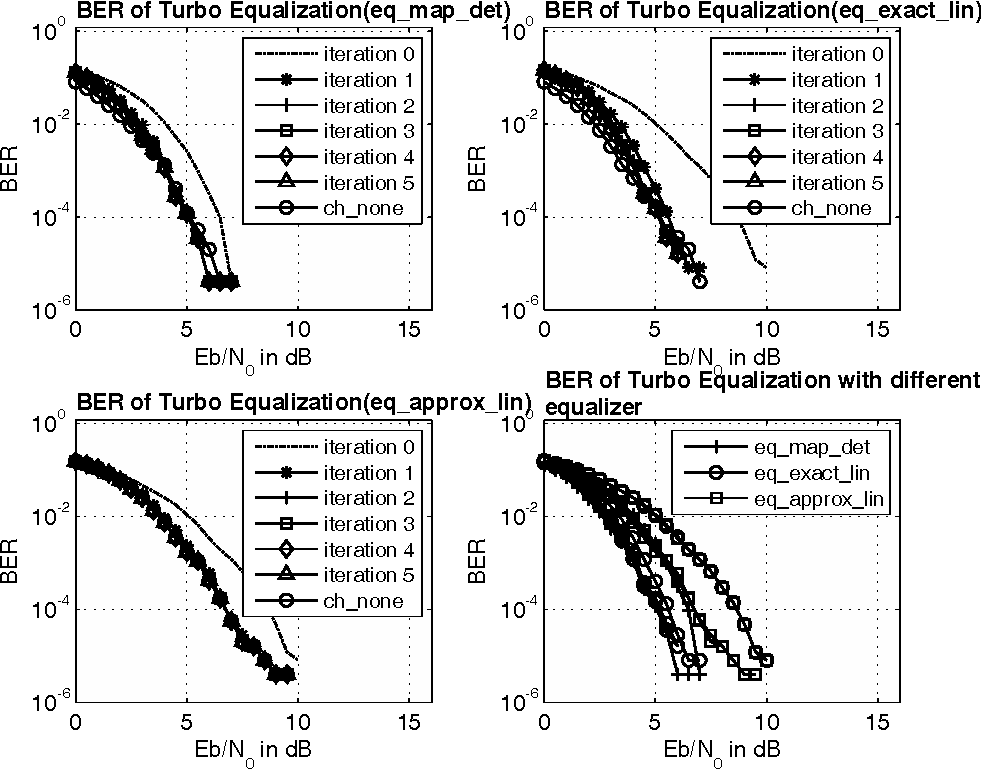
\includegraphics[width=\textwidth]{images/different_equalizers_separate.pdf}
  \end{center}
  \caption{不同均衡算法的性能比较}
  \label{fig:3.3}
\end{figure}
可以从两方面分析图\ref{fig:3.3},
\begin{enumerate}
    \item
        单独分析每一个图,可以看出,随着迭代次数的增加,所有均衡算法的误码率曲线都越来越接近AWGN下的误码率曲线。这说明,随着迭代次数的增加,外部信息被利用的越来越充分。
    \item
        分析图\ref{fig:3.3}中最后一个小图,可以看出,MAP均衡算法是最好的,但是随着迭代次数的增加,MMSE算法以及其近似算法越来越接近MAP均衡性能。因此,用基于先验信息MMSE准则的线性Turbo均衡算法代替MAP算法对性能的损失很小。
\end{enumerate}

\subsection{不同调制方式之间的比较}
\begin{longtable}{|c||c|c|}
  \caption{不同调制方式均衡性能比较的参数设置}
  \label{tab:3.7}\\

  \endfirsthead

  \multicolumn{3}{c}{续表~\thetable\hskip1em 不同调制方式均衡性能比较的参数设置}

  \endhead
  
  \hline
  \multicolumn{3}{r}{续下页}
  \endfoot
  \endlastfoot
    \hline
    \multicolumn{2}{|c|}{参数项}&参数值\\
    \hline
    &ch\_none&无码间干扰\\
    \cline{2-3}
   \raisebox{2.3ex}[0pt]{信道类型}&CHA&$[0.407 \;0.815\; 0.407]$\\
   \hline
   均衡类型&eq\_exact\_lin&MMSE精确线性均衡算法\\
   \hline
    &\textbf{mo\_bpsk}&\textbf{BPSK}\\
   \cline{2-3}
   \textbf{调制方式}&\textbf{mo\_qpsk}&\textbf{QPSK}\\
   \cline{2-3}
   &\textbf{mo\_8psk}&\textbf{8PSK}\\
   \hline
   交织长度&bl\_1024&1024\\
   \hline
   编码长度&co\_r2\_m2&$[5\; 7]$\\
   \hline
   删余方式&pu\_1&无删余\\
   \hline
   编码类型&RSC&递归系统卷积码\\
    \hline
\end{longtable}
参数如表\ref{tab:3.7},仿真结果如图\ref{fig:3.4}
\begin{figure}[htb]
  \begin{center}
    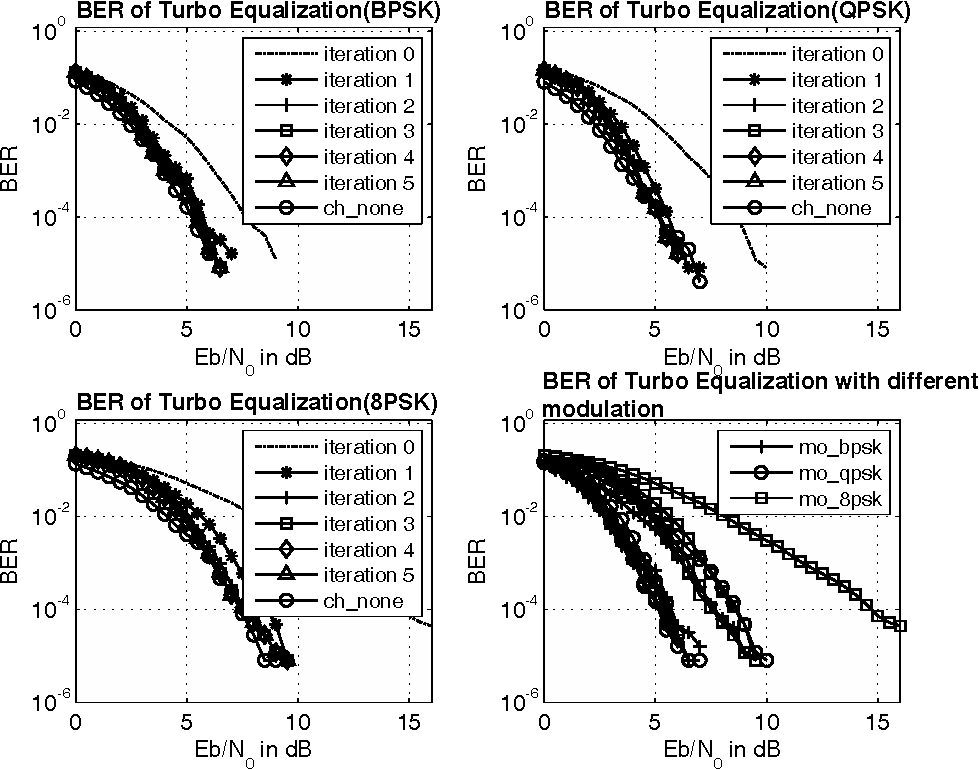
\includegraphics[width=\textwidth]{images/different_mod_separate.pdf}
  \end{center}
  \caption{不同调制方式下均衡性能的比较}
  \label{fig:3.4}
\end{figure}
可以从两方面分析图\ref{fig:3.4},
\begin{enumerate}
    \item
        单独分析每一个图,可以看出,随着迭代次数的增加,所有调制方式下的误码率曲线都越来越接近AWGN下的误码率曲线。这说明,随着迭代次数的增加,外部信息被利用的越来越充分。
    \item
        分析图\ref{fig:3.4}中最后一个小图,可以看出,BPSK的性能最好,QPSK的性能次之,最差的是8PSK,究其原因,8PSK调制下的码字之间的欧式距离最小,最容易出错,因此性能最差,但是8PSK的码率最高,在实际应用中要综合考虑性能和码率之间的平衡。本文所在的水声相干通信系统中综合考虑这两方面,采用的是QPSK调制方式。
\end{enumerate}

\subsection{不同编码方式之间的比较}
\begin{longtable}{|c||c|c|}
  \caption{不同编码方式均衡性能比较的参数设置}
  \label{tab:3.8}\\

  \endfirsthead

  \multicolumn{3}{c}{续表~\thetable\hskip1em 不同编码方式均衡性能比较的参数设置}

  \endhead
  
  \hline
  \multicolumn{3}{r}{续下页}
  \endfoot
  \endlastfoot
    \hline
   \multicolumn{2}{|c|}{参数项}&参数值\\
   \hline
    &ch\_none&无码间干扰\\
    \cline{2-3}
   \raisebox{2.3ex}[0pt]{信道类型}&CHA&$[0.407\; 0.815\; 0.407]$\\
   \hline
   均衡类型&eq\_exact\_lin&MMSE精确线性均衡算法\\
   \hline
   调制方式&mo\_bpsk&BPSK\\
   \hline
   交织长度&bl\_1024&1024\\
   \hline
   &\textbf{co\_r2}\_m2&$\mathbf{[5\; 7]}$\\
   \cline{2-3}
   \raisebox{2.3ex}[0pt]{\textbf{编码方式}}&\textbf{co\_r2\_m4}&$\mathbf{[19\;
   29]}$\\
   \hline
   删余方式&pu\_1&无删余\\
   \hline
   编码类型&RSC&递归系统卷积码\\
    \hline
\end{longtable}
参数如表\ref{tab:3.8},仿真结果如图\ref{fig:3.5}
\begin{figure}[htb]
  \begin{center}
    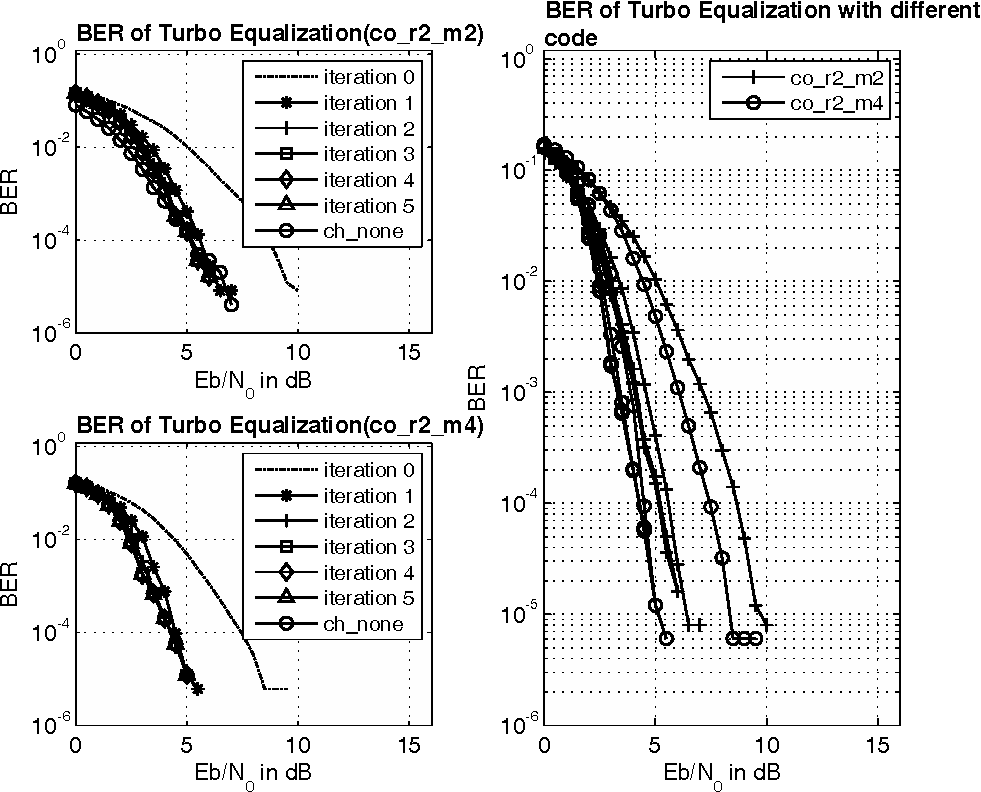
\includegraphics[width=\textwidth]{images/different_code_separate.pdf}
  \end{center}
  \caption{不同调制方式下均衡性能的比较}
  \label{fig:3.5}
\end{figure}
可以从两方面分析图\ref{fig:3.5},
\begin{enumerate}
    \item
        单独分析每一个图,可以看出,随着迭代次数的增加,所有编码方式下的误码率曲线都越来越接近AWGN下的误码率曲线。这说明,随着迭代次数的增加,外部信息被利用的越来越充分。
    \item
        分析图\ref{fig:3.5}中最后一个小图,可以看出,约束长度越大的编码方式,其性能越好(每一次迭代的比较结果,都是约束长度大的编码方式更优)。因为约束长度越大的编码方式,其译码性能越好,反馈给均衡器的外部信息越准确,因此,总体的译码性能会越好。考虑到这个问题,本文在湖试数据处理部分采用的是纠错性能极强的Turbo码。
\end{enumerate}

\subsection{不同删余方式之间的比较}
\begin{longtable}{|c||c|c|}
  \caption{不同删余方式均衡性能比较的参数设置}
  \label{tab:3.9}\\

  \endfirsthead

  \multicolumn{3}{c}{续表~\thetable\hskip1em 不同删余方式均衡性能比较的参数设置}

  \endhead
  
  \hline
  \multicolumn{3}{r}{续下页}
  \endfoot
  \endlastfoot
    \hline
   \multicolumn{2}{|c|}{参数项}&参数值\\
   \hline
    &ch\_none&无码间干扰\\
    \cline{2-3}
   \raisebox{2.3ex}[0pt]{信道类型}&CHA&$[0.407\; 0.815\; 0.407]$\\
   \hline
   均衡类型&eq\_exact\_lin&MMSE精确线性均衡算法\\
   \hline
   调制方式&mo\_bpsk&BPSK\\
   \hline
   交织长度&bl\_1024&1024\\
   \hline
   编码方式&co\_r2\_m2&$[5\; 7]$\\
   \hline
   &\textbf{pu\_1}&\textbf{无删余}\\
   \cline{2-3}
   \raisebox{2.3ex}[0pt]{\textbf{删余方式}}&\textbf{pu\_100}&$\mathbf{3/4}$\\
   \hline
   编码类型&RSC&递归系统卷积码\\
    \hline
\end{longtable}
参数如表\ref{tab:3.9},仿真结果如图\ref{fig:3.6}
\begin{figure}[htb]
  \begin{center}
    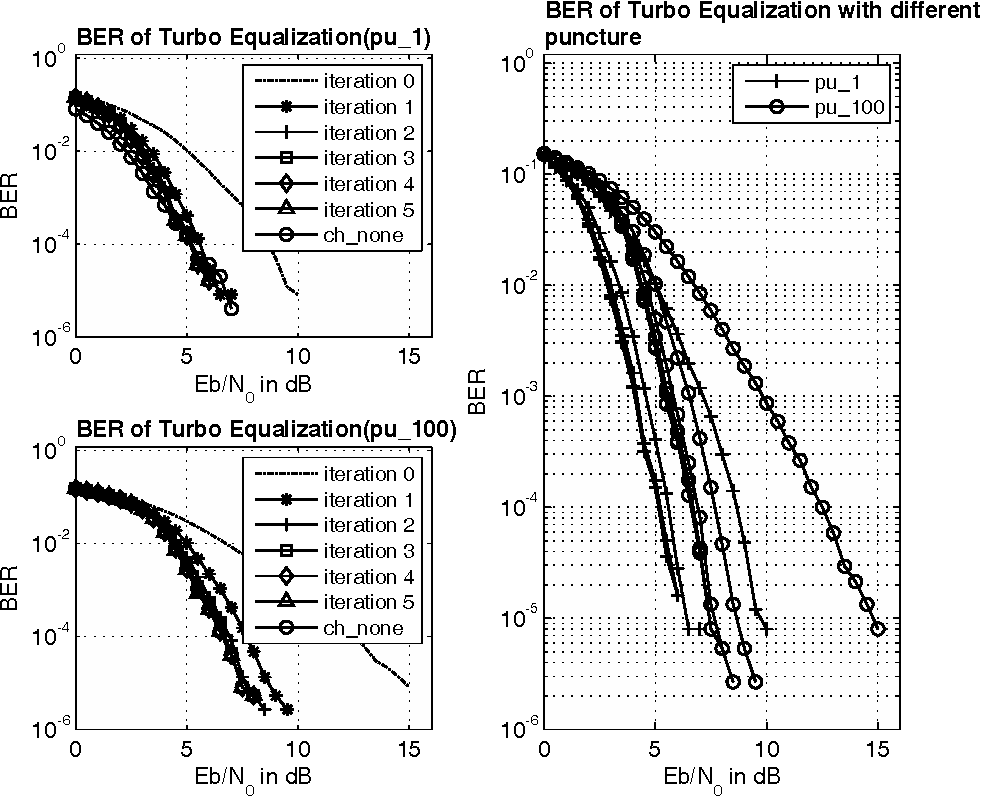
\includegraphics[width=\textwidth]{images/different_puncture_separate.pdf}
  \end{center}
  \caption{不同删余方式下均衡性能的比较}
  \label{fig:3.6}
\end{figure}
可以从两方面分析图\ref{fig:3.6},
\begin{enumerate}
    \item
        单独分析每一个图,可以看出,随着迭代次数的增加,所有删余方式下的误码率曲线都越来越接近AWGN下的误码率曲线。这说明,随着迭代次数的增加,外部信息被利用的越来越充分。
    \item
        分析图\ref{fig:3.6}中最后一个小图,可以看出,删余越小,其性能越好(每一次迭代的比较结果,都是删余小的均衡性能更优)。因为删余越小,损失的信息越少,其译码性能越好,反馈给均衡器的外部信息越准确,因此,总体的译码性能会越好。但是删余越少,其码率越低,考虑到这个问题,本文在湖试数据处理部分采用的删余方式为pu\_100。
\end{enumerate}

\subsection{不同交织长度之间的比较}
\begin{longtable}{|c||c|c|}
  \caption{不同交织长度均衡性能比较的参数设置}
  \label{tab:3.10}\\

  \endfirsthead

  \multicolumn{3}{c}{续表~\thetable\hskip1em 不同交织长度均衡性能比较的参数设置}

  \endhead
  
  \hline
  \multicolumn{3}{r}{续下页}
  \endfoot
  \endlastfoot
    \hline
   \multicolumn{2}{|c|}{参数项}&参数值\\
   \hline
    &ch\_none&无码间干扰\\
    \cline{2-3}
   \raisebox{2.3ex}[0pt]{信道类型}&CHA&$[0.407\; 0.815\; 0.407]$\\
   \hline
   均衡类型&eq\_exact\_lin&MMSE精确线性均衡算法\\
   \hline
   调制方式&mo\_bpsk&BPSK\\
   \hline
   &\textbf{bl\_1024}&\textbf{1024}\\
   \cline{2-3}
   \raisebox{2.3ex}[0pt]{\textbf{交织长度}}&\textbf{bl\_65535}&\textbf{65535}\\
   \hline
   编码方式&co\_r2\_m2&$[5 \;7]$\\
   \hline
   删余方式&pu\_1&无删余\\
   \hline
   编码类型&RSC&递归系统卷积码\\
    \hline
\end{longtable}
参数如表\ref{tab:3.10},仿真结果如图\ref{fig:3.7}
\begin{figure}[htb]
  \begin{center}
    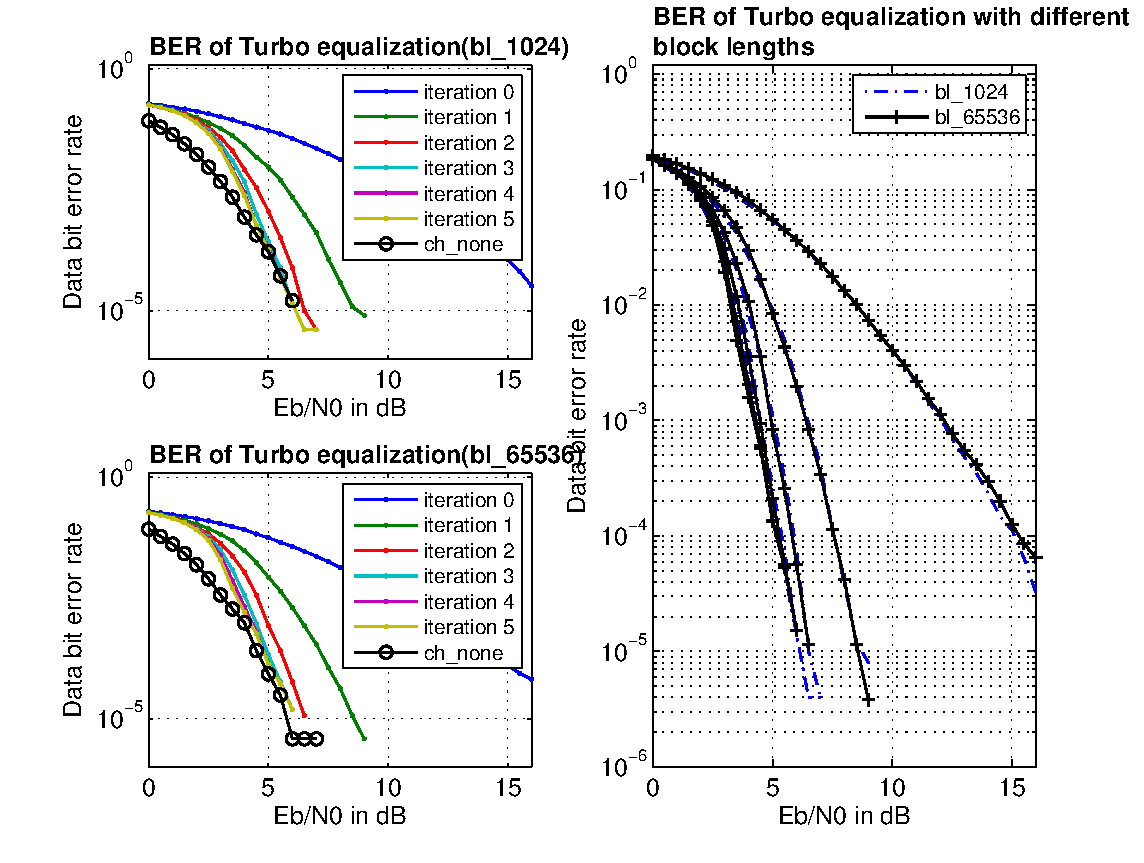
\includegraphics[width=\textwidth]{images/different_block_length_separate.pdf}
  \end{center}
  \caption{不同调制方式下均衡性能的比较}
  \label{fig:3.7}
\end{figure}
可以从两方面分析图\ref{fig:3.7},
\begin{enumerate}
    \item
        单独分析每一个图,可以看出,随着迭代次数的增加,所有交织长度下的误码率曲线都越来越接近AWGN下的误码率曲线。这说明,随着迭代次数的增加,外部信息被利用的越来越充分。
    \item
        分析图\ref{fig:3.7}中最后一个小图,两种交织长度下的均衡性能基本一致,这是因为,在交织长度很小的情况下,随着交织长度的增加,均衡和译码的性能都会有所提升,但是当交织长度增大到一定值之后,再增加交织长度并不会提高均衡和译码性能,而相反会增加均衡和译码的计算量。综合考虑这个问题,本文在湖试数据处理部分采用的交织长度为1936。
\end{enumerate}

\section{分数间隔线性SISO均衡算法}
上面介绍的都是采用符号采样率的均衡器,这在多普勒比较严重的水声信道中容易产生相位翻转的现象,为了解决这个问题,通常采用分数间隔均衡器,下面将介绍采样率为二倍符号率的线性SISO均衡算法。

当接收信号采用二倍符号速率采样时,接收符号可以改写为:
\begin{eqnarray}
    z_{n,i}=\sum_{l=0}^{M-1}h_{n,l,i}x_{n-l}+\omega_{n,i},\;i\in\{0,1\}
    \label{equ:3.38}
\end{eqnarray}
其中$\mathbf{h}_{n,i}=[h_{n,0,i},\cdots,h_{n,M-1,i}]^{\mathrm{T}}$为分数间隔时变信道冲激响应。依然假设$N$为符号速率均衡器长度,那么真实的均衡器(分数间隔均衡器)长度为$2N$,因此,为了计算此时的发送符号的估计值$\hat{x}_n$,需要知道$2N$个长度的接收符号$z_{n,i}$以及$N+M-1$个长度的关于发送符号$x_n$的先验信息。重新定义向量$\mathbf{z}_n$和$\boldsymbol{\omega}_n$,使其长度为$2N$。
\begin{eqnarray}
    \begin{array}{l@{\;=\;}l}
        \mathbf{z}_n&[z_{n+\mathrm{N}_1,1},z_{n+\mathrm{N}_1,0},z_{n+\mathrm{N}_1-1,1},\cdots,z_{n-\mathrm{N}_2,1},z_{n-\mathrm{N}_2,0}]^{\mathrm{T}}\\
        \boldsymbol{\omega}_n&[\omega_{n+\mathrm{N}_1,1},\omega_{n+\mathrm{N}_1,0},\omega_{n+\mathrm{N}_1-1,1},\cdots,\omega_{n-\mathrm{N}_2,1},\omega_{n-\mathrm{N}_2,0}]^{\mathrm{T}}
    \end{array}
    \label{equ:3.39}
\end{eqnarray}

此时的信道卷积矩阵的大小为$2N\times(N+M-1)$:
\begin{eqnarray}
    \begin{array}{l@{\;=\;}l}
        \mathbf{H}_n&
        \begin{bmatrix}
            \mathbf{h}_{n+\mathrm{N}_1,1}^{\mathrm{T}}&0&\cdots&0\\
            \mathbf{h}_{n+\mathrm{N}_1,0}^{\mathrm{T}}&0&\cdots&0\\
            0&\mathbf{h}_{n+\mathrm{N}_1,1}^{\mathrm{T}}&\cdots&0\\
            0&\mathbf{h}_{n+\mathrm{N}_1,0}^{\mathrm{T}}&\cdots&0\\
           &\cdots&&\\ 
            0&&\cdots&\mathbf{h}_{n+\mathrm{N}_1,1}^{\mathrm{T}}\\
            0&\qquad&\cdots&\mathbf{h}_{n+\mathrm{N}_1,0}^{\mathrm{T}}\\
        \end{bmatrix}\\
        &\begin{bmatrix}
            h_{n+\mathrm{N}_1,0,1}&h_{n+\mathrm{N}_1,1,1}&\cdots&h_{n+\mathrm{N}_1,\mathrm{M}-1,1}&0&\cdots&0\\
            h_{n+\mathrm{N}_1,0,0}&h_{n+\mathrm{N}_1,1,0}&\cdots&h_{n+\mathrm{N}_1,\mathrm{M}-1,0}&0&\cdots&0\\
            0&h_{n+\mathrm{N}_1-1,0,1}&\cdots&h_{n+\mathrm{N}_1-1,\mathrm{M}-1,1}&0&\vdots\\
            0&h_{n+\mathrm{N}_1-1,0,0}&\cdots&h_{n+\mathrm{N}_1-1,\mathrm{M}-1,0}&0&\vdots\\
            \vdots&&\ddots&&0\\
            0&\cdots&0&h_{n-\mathrm{N}_2,0,1}&h_{n-\mathrm{N}_2,1,1}&\cdots&h_{n-\mathrm{N}_2,\mathrm{M}-1,1}\\
            0&\cdots&0&h_{n-\mathrm{N}_2,0,0}&h_{n-\mathrm{N}_2,1,0}&\cdots&h_{n-\mathrm{N}_2,\mathrm{M}-1,0}\\
        \end{bmatrix}
    \end{array}
    \label{equ:3.40}
\end{eqnarray}

假设噪声的方差$\sigma_{\omega,n,i}^2=\mathrm{E}(\omega_{n,i},\omega_{n,i}^*)$在每一个符号都是不同的,而且是独立的,因此噪声的协方差矩阵$\boldsymbol{\Omega}_n=\mathrm{Cov}(\boldsymbol{\omega}_n,\boldsymbol{\omega}_n)$为:
\begin{eqnarray}
    \boldsymbol{\Omega}_n=\mathrm{diag}[\sigma_{\omega,n+\mathrm{N}_1,1}^2,\sigma_{\omega,n+\mathrm{N}_1,0}^2,\cdots,\sigma_{\omega,n-\mathrm{N}_2,1}^2,\sigma_{\omega,n-\mathrm{N}_2,0}]
    \label{equ:3.41}
\end{eqnarray}
有了以上的改写,接收符号序列为:
\begin{eqnarray}
    \mathbf{z}_n=\mathbf{H}_n\mathbf{x}_n+\boldsymbol{\omega}
    \label{equ:3.42}
\end{eqnarray}

此时,接收符号的表达式与非分数间隔SISO均衡器的接收符号表达式是一致的,因此,可以利用非分数间隔均衡器的算法来求解分数间隔均衡器,只是矩阵的维数为$2N\times
2N$而不是原来的$N\times N$。

为了避免计算矩阵的逆,依然采用类似与3.1.1节中的时间递归更新算法。定义$\boldsymbol{\Sigma}_n=\mathbf{H}_n\mathrm{V}_n\mathbf{H}_n^{\mathrm{H}}+\boldsymbol{\Omega}_n$和$\mathbf{U}_n=\boldsymbol{\Sigma}_n^{-1}$,其维度为$2N\times
2N$。与3.1.1。节不同,此时对$\boldsymbol{\Sigma}_n$和$\mathbf{U}_n$划分的四个部分都是矢量,为了方便区分,这里采用与3.1.1节不同的符号表示:
\begin{eqnarray}
    \begin{array}{c}
        \boldsymbol{\Sigma}_{n-1}=
        \begin{bmatrix}
            \mathbf{A}_n&\mathbf{G}_n\\
            \mathbf{G}_n^{\mathrm{H}}&\mathbf{B}_n\\
        \end{bmatrix},\;
        \boldsymbol{\Sigma}_n=
        \begin{bmatrix}
            \mathbf{E}_n&\mathbf{F}_n^{\mathrm{H}}\\
            \mathbf{F}_n&\mathbf{A}_n\\
        \end{bmatrix}\\
        \mathbf{U}_{n-1}=
        \begin{bmatrix}
            \mathbf{D}_n&\mathbf{N}_n\\
            \mathbf{N}_n^{\mathrm{H}}&\mathbf{M}_n\\
        \end{bmatrix},\;
        \mathbf{U}_n=
        \begin{bmatrix}
            \mathbf{K}_n&\mathbf{L}_n^{\mathrm{H}}\\
            \mathbf{L}_n&\mathbf{C}_n\\
        \end{bmatrix}\\
    \end{array}
    \label{equ:3.43}
\end{eqnarray}
其中,$\mathbf{B}_n\mbox{,}\mathbf{E}_n\mbox{和}\mathbf{M}_n$都是$2\times
2$的矩阵,$\mathbf{F}_n\mbox{,}\mathbf{G}_n\mbox{,}\mathbf{L}_n\mbox{和}\mathbf{N}_n$都是$(2N-2)\times
2$的矩阵,$\mathbf{A}_n\mbox{,}\mathbf{C}_n\mbox{和}\mathbf{D}_n$都是$(2N-2)\times(2N-2)$的矩阵。整体思路与3.1.1节一样,通过求解$\boldsymbol{\Sigma}_n\mathbf{U}_n=\boldsymbol{\Sigma}_{n-1}\mathbf{U}_{n-1}=\mathbf{I}_{2\mathrm{N}}$,也就是
\begin{eqnarray}
    \begin{array}{l@{\;=\;}l}
        \mathbf{A}_n\mathbf{D}_n+\mathbf{G}_n\mathbf{N}_n^{\mathrm{H}}&\mathbf{I}_{2\mathrm{N}-2}\\
        \mathbf{A}_n\mathbf{D}_n+\mathbf{G}_n\mathbf{M}_n&\mathbf{0}_{2\mathrm{N}-2}\\
        \mathbf{E}_n\mathbf{K}_n+\mathbf{F}_n^{\mathrm{H}}\mathbf{L}_n&\mathbf{I}_2\\
        \mathbf{F}_n\mathbf{K}_n+\mathbf{A}_n\mathbf{L}_n&\mathbf{0}_{2\mathrm{N}-2}\\
        \mathbf{F}_n\mathbf{L}_n^{\mathrm{H}}+\mathbf{A}_n\mathbf{C}_n&\mathbf{I}_{2\mathrm{N}-2}
    \end{array}
    \label{equ:3.44}
\end{eqnarray}
可以得到$\mathbf{C}_n\mbox{,}\mathbf{K}_n\mbox{和}\mathbf{L}_n$,然后结合$\mathbf{U}_{n-1}\mbox{,}\mathbf{E}_n\mbox{和}\mathbf{F}_n$可以得到$\mathbf{U}_n$:
\begin{eqnarray}
    \begin{array}{l@{\;=\;}l}
        \mathbf{A}_{n}^{-1}&\mathbf{D}_n-\mathbf{N}_n\mathbf{M}_n^{-1}\mathbf{N}_n^{\mathrm{H}}\\
        \boldsymbol{\Psi}_n&\mathbf{A}_n^{-1}\mathbf{F}_n\\
        \mathbf{K}_n&(\mathbf{E}_n-\mathbf{F}_n^{\mathrm{H}}\boldsymbol{\Psi}_n)^{-1}\\
        \mathbf{L}_n&-\boldsymbol{\Psi}_n\mathbf{K}_n\\
        \mathbf{C}_n&\mathbf{A}_n^{-1}+\boldsymbol{\Psi}_n\mathbf{K}_n\boldsymbol{\Psi}_n^{\mathrm{H}}
    \end{array}
    \label{equ:3.45}
\end{eqnarray}
此算法与上文中的符号间隔更新算法是一致的,当利用式\ref{equ:3.45}求解出$\mathbf{U}_n$之后,就可以用同样的方法求解$\mathbf{f}_n$和${\mathbf{f}}'_n$。

需要说明一下,本文在仿真的时候并没有实现分数间隔MMSE均衡算法,而是在湖试数据处理部分直接应用此算法。
\section{Turbo均衡与Turbo联合迭代}
从上面的仿真分析可以看出,不论采用何种均衡算法(MAP,MMSE-optimal,MMSE-LC)都不能达到AWGN信道下的性能。而上文中的仿真采用的是卷积码,因此为了获得更好的均衡性能,可以采用纠错性能极好的Turbo码来代替卷积码。

当turbo均衡中引用turbo码作为系统的差错控制编码时,发送端需要两个交织器,一个交织器是用于两个分量编码器之间,另一个交织器是用于编码器与符号映射器/信道之间。在接收端,不考虑软迭代信道估计算法,总共有两处迭代回路,一处是两个SISO分量译码器之间的迭代,一处是SISO译码器与SISO均衡器的迭代。具体可以参考\ncite{Raphaeli1997,xiang2003,Yeap2002,Hanzo2002,Yang2007,Yang2005}。

传统的结合Turbo码的Turbo均衡算法是在一次均衡迭代之中,Turbo码本身进行了多次迭代,但文献\ncite{FonsecadosSantos2007}中提出一种新的关于均衡与译码之间迭代调度算法。在每一次均衡迭代中,只和Turbo译码器中的一个分量译码器进行迭代,而分量译码器之间交互信息是通过均衡器的迭代,相当于传统的算法是均衡器迭代为外部迭代,而译码器迭代为内部迭代,而文献\ncite{FonsecadosSantos2007}中将译码器迭代作为外部迭代而均衡器迭代作为内部迭代。此算法的优点是降低了复杂度。
\section{采用预编码的线性SISO均衡算法}
在前面介绍的迭代均衡和译码的主要思想是在均衡器和译码器之间通过传递软信息以迭代的方式进行联合译码检测。如果把卷积码和ISI信道看作是一个串行级联的卷积码(SCCC)\cite{Benedetto1998},则卷积码就是外码,而把ISI信道看做是内码。在文\ncite{Benedetto1998}中显示,对于串行级联码仅作为内码是递归卷积码,级联码才有交织增益,而ISI信道是典型的有限脉冲响应(FIR)等效于一个非递归的卷积码,因此,不会获得交织增益,只能通过提高外码编码器的性能改善。

在本节研究通过采用二进制预编码技术,可以使得信道“表现”出递归特性,获得良好的交织增益。作为外码的卷积码编码器就可以使用小的约束长度实现高的编码增益,同时也降低了译码复杂度(与卷积码约束长度相关)。

预编码的记忆长度要小于信道的记忆长度,这样通过二进制预编码后不改变网格状态数,因而并不增加线性均衡器复杂度,而最常用的是查分结构的预编码。
\begin{figure}[htb]
  \begin{center}
    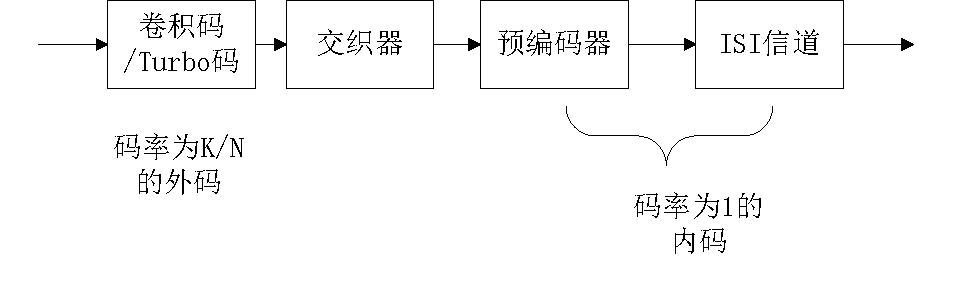
\includegraphics[width=0.8\textwidth]{images/diffcoder.pdf}
  \end{center}
  \caption{采用预编码的串行级联模型}
  \label{fig:3.8}
\end{figure}

文献\ncite{Daly2010}指出,采用预编码后,在低信噪比下,比没采用预编码的线性均衡器性能下降,是由于差错传播的原因。但是随着信噪比的增加,从误码率的下降斜率可以看出,由于获得了交织增益,性能取得了非常明显的改善,甚至比AWGN下的性能有$1-2\mbox{dB}$的增益。

但是考虑到水声通信系统的实际情况,需要保证低信噪比下的信息传输的有效性,而预编码方案在低信噪比下性能反而会更差一些,不满足需求,综合考虑,本文在湖试数据处理的时候采用的Turbo码与MMSE-LE级联的均衡迭代方案。
\section{本章小结}
本章详细介绍了基于先验信息MMSE准则的线性Turbo均衡算法以及其近似算法,并为了避免矩阵求逆的操作,介绍了一种递归更新算法,使得运算复杂度大大减少。文中对介绍算法进行仿真,并分析该算法的优劣之处。

简单介绍了基于先验信息MMSE准则的线性Turbo均衡算法与Turbo码联合迭代,并给出几个参考。介于水声通信系统中相位变化的情况,介绍了该算法的分数间隔实现方式,用以解决相位翻转问题。

本章最后介绍了在发送端可以加入预编码来提高均衡性能,但是针对水声相干通信的特点,本文并没有采用这种方案。
%%========================================================================
% empty page for two-page print
%\ifthenelse{\equal{\ioaside}{T}}{%
%  \newpage\mbox{}%
%  \thispagestyle{empty}}{}
%%========================================================================
%\end{document}
\clearpage{\pagestyle{empty}\cleardoublepage}